\input{../header.tex}

\subject{VERSUCH NUMMER 700}
\title{Natürliche Relativität}
\date{
  Durchführung: 30.05.2023
  \hspace{3em}
  Abgabe: 06.06.2023
}

\begin{document}

\maketitle
\thispagestyle{empty}
\tableofcontents
\newpage
\setcounter{page}{1}
\section{Ziel}
\label{sec:Ziel}
Das Ziel dieses Versuches ist es verschiedene Stoffe auf radioaktive Aktivität zu untersuchen und Aussagen über die emittierte Strahlungsart zu treffen. 
\section{Theorie}
\label{sec:Theorie}


\section{Aufbau}
\label{sec:Aufbau}


\section{Durchführung}
\label{sec:Durchführung}


\section{Auswertung}
\label{sec:Auswertung}

%\subsection{Fehlerrechnung}
\label{sec:Fehlerrechnung}
Für die Fehlerrechnung werden folgende Formeln aus der Vorlesung verwendet.
für den Mittelwert gilt
\begin{equation}
    \overline{x}=\frac{1}{N}\sum_{i=1}^N x_i ß\; \;\text{mit der Anzahl N und den Messwerten x} 
    \label{eqn:Mittelwert}
\end{equation}
Der Fehler für den Mittelwert lässt sich gemäß
\begin{equation}
    \increment \overline{x}=\frac{1}{\sqrt{N}}\sqrt{\frac{1}{N-1}\sum_{i=1}^N(x_i-\overline{x})^2}
    \label{eqn:FehlerMittelwert}
\end{equation}
berechnen.
Wenn im weiteren Verlauf der Berechnung mit der fehlerhaften Größe gerechnet wird, kann der Fehler der folgenden Größe
mittels Gaußscher Fehlerfortpflanzung berechnet werden. Die Formel hierfür ist
\begin{equation}
    \increment f= \sqrt{\sum_{i=1}^N\left(\frac{\partial f}{\partial x_i}\right)^2\cdot(\increment x_i)^2}.
    \label{eqn:GaussMittelwert}
\end{equation}
Alle Messwerte werden im folgenden für ein Zeitintervall von einer Sekunde angegeben, sodass diese direkt die Aktivität der Probe darstellen.

Die gemessene Untergrundrate ergibt sich zu
\begin{equation*}
    (0.582 \pm 0.241) \,\unit{\becquerel} \; .
\end{equation*}
Dabei wird die Standardabweichung über 
\begin{equation}
    \sigma = \sqrt{N}
    \label{eqn:standardabweichung}
\end{equation}
berechnet. Auch bei allen weiteren Messungen ergibt sich die Fehlerabweichung über \autoref{eqn:standardabweichung}
Die Hintergrundrate muss von allen weiteren Messungen abgezogen werden.

Zur Abschätzung der Zerfallsart wird zur Grundlage genommen, dass sämtliche $\alpha$-Strahlung bereist eine dünne Schutzkappe blockiert werden und die Abschrimung von $\beta$-Strahlen durch
die Aluminiumplatte erfolgt, sodass nach Einfügen der Platte einzig die $\gamma$-Strahlung detektiert werden kann.

\subsection{Natürliche radioaktive Stoffe}
\label{sec:stoffe}
In der ersten Messung wird die Aktivität von Paranüssen, dessen Masse $m = 17.45 \, \unit{\gram}$ beträgt, bestimmt. Dazu wurde fünfmal für das Zeitintervall 
von einer Minute gemessen. Wenn alle Messwerte aufaddiert und dann für das Intervall von einer Sekunde angegeben werden, ergibt sich 
\begin{equation*}
    (7.4667 \pm 2.7325) \, \unit{\becquerel} \; .
\end{equation*}
Von diesem  Wert muss nun noch die Hintergrundstrahlung abgezogen werden, sodass sich die Aktivität von Paranüssen zu 
\begin{equation*}
    A_{\symup{Paranuss}} = (1.65 \pm 1.28) \, \unit{\becquerel} 
\end{equation*}
ergibt. Desweiteren kann die spezifische Aktivität über
\begin{equation}
    a = \frac{A}{m}
    \label{eqn:spezAkt}
\end{equation}
berechnet werden. Bei Paranüssen ergibt sich diese mit der oben angegebenen Masse zu 
\begin{equation*}
    a_{{\symup{Paranuss}}} = (94.56 \pm 9.72) \, \unit{\becquerel \per \kilo\gram} \; .
\end{equation*}

Um die Art der Strahlung zu bestimmen wurde zuerst mit der Schutzkappe abgeschirmt. Es werden noch 33 Zerfälle pro Minute gezählt. Das heißt es werden
$26.34 \, \%$ der Strahlung abgeschirmt. Dies ist der Anteil der Alphastrahlung. Bei der Abschirmung mit der Aluminiumplatte werden noch 29 
Zerfälle pro Minute detektiert. Daraus lässt sich schließen, dass der Anteil der Betastrahlung bei $8.93 \,\%$ liegt.

Bei der zweiten Messung wird die Aktivität von Blaukorn, mit einer Masse $24.42\,\unit{\gram}$, einmal für ein Zeitintervall von zehn Minuten gemessen.
Diese Messung wird nun für den Zeitraum von einer Sekunde angegeben
\begin{equation*}
    (33.10 \pm 5.75) \,\unit{\becquerel} \; .
\end{equation*}
Auch hier wird wieder die Hintergrundrate abgezogen. Die Aktivität ergibt sich zu 
\begin{equation*}
    A_{\symup{Blaukorn}} = (27.28 \pm 5.22) \, \unit{\becquerel} \; .
\end{equation*}
Des Weiteren wird die spezifische Aktivität mittels \autoref{eqn:spezAkt} zu 
\begin{equation*}
    a_{\symup{Blaukorn}} = (1117.25 \pm 33.43) \,\unit{\becquerel \per \kilo\gram}
\end{equation*} 
bestimmt. 

Bei der Abschirmung mit Hilfe der Schutzkappe werden noch 45 Zerfälle pro Minute detektiert, sodass sich ein Anteil der Alphastrahlung von $77.34 \,\%$ 
ergibt. Bei Abschirmung mit der Aluminiumplatte werden noch 34 Zerfälle pro Minute gezählt. Damit ergibt sich der Anteil der Betastrahlung zu 
$6.06 \,\%$ ergibt.

\subsection{Radioaktivität in der Raumluft}
\label{sec:Radioaktivität in der Raumluft}

Die mit dem Geiger-Müller-Zählrohr sind in der \autoref{tab:loon} dargestellt.

\begin{table}
    \centering 
    \caption{Gemessene Zerfälle pro Minute des ungefüllten Ballons.}
    \begin{tabular}{c c c}
        \toprule
        Messung & Anzahl $N$ der Zerfälle pro Minute\\
        \midrule
        1 & 31 \\
        2 & 35 \\
        3 & 39 \\
        4 & 41 \\
        5 & 24 \\
    \end{tabular}
\end{table}
Daraus ergibt sich ein MIttelwert mit einer aus der Standardabweichung resultierender Abweichung von
\begin{equation*}
    \bar{N}= 34\pm 5.83\, .
\end{equation*}
Hier ist zu erwähnen, dass von einer Anzahl gesprochen wird und somit Dezimalstellen keinen Sinn ergeben. Jedoch wird hier diese angegeben und in weiteren 
Berechnungen verwendet, um den Rundungsfehler möglichst gering zu halten.
Für die Aktivität folgt so nach \autoref{eqn:Aktivität}
\begin{equation*}
    A= (0.57\pm 0.10)\, \text{Bq}\, .
\end{equation*}
Abzüglich der Hintergrundstrahlung ergibt sich so eine Aktivität von
\begin{equation*}
    A_{\text{luftleerer Ballon}}= (-0.02\pm 0.26)\, \text{Bq}\, .
\end{equation*}
Eine negative Aktivität ist physikalisch nicht möglich, aber es geht hervor, dass durch den Ballon ein Teil der Hintergrundstrahlung abgeschirmt wird.

Nachdem der aufgeblasene und ionisierte Ballon einige Zeit im strahlungsreicheren Keller verbracht hat, wurde binnen einer 5 minütigen Messung eine Anzahl
von 
\begin{equation*}
    N= 5986.00 \pm 77.37
\end{equation*} 
Daraus folgt eine Aktivität von
\begin{equation*}
    A= (19.95 \pm 0.26) \, \text{Bq}\, .
\end{equation*}
Für die bereinigte Aktivität folgt so 
\begin{equation*}
    A_{\text{aufgeblasener Ballon}}= (19.37\pm 0.35) \, \text{Bq}\, .
\end{equation*}
Nach der Installation der Schutzkappe, wurden in einem Intervall von einer Minute noch 162 Zerfälle detektiert und mit einer Aluminiumplatte 43.
Bei der Messung ohne Abschirmung hingegen konnten 1197 Zerfälle pro Minute detektiert werden.
Somit wurde nach der Installation der Abdeckung nur noch $13.53\%$ der ursprünglichen Zerfälle registriert.
Das Hinzufügen einer Aluminiumplatte verringerte diese Anteil weiter  auf $3.59\%$ des Ursprungswertes.
Es kann unter Betrachtung der Abnahme der Zerfälle gefolgert werden, dass $86.47\%$ der detektierten Strahlung $\alpha$-Strahlung war.
Analog kann festgehalten werden, dass $3.59\%$ der Starhlung auf $\gamma$-Strahlung zurückgeführt werden kann.
\section{Diskussion}
\label{sec:Diskussion}

Die in \autoref{sec:stoffe} berechneten spezifischen Aktivitäten werden nun mit theoretischen Werten verglichen. Für Paranüsse ergibt sich für die spezifische 
Aktivität ein Wert zwischen $8\,\unit{\becquerel\per\kilo\gram}$ und $130\,\unit{\becquerel\per\kilo\gram}$ \cite{ap700}. Der experimentell bestimmte Wert 
$94.56\,\unit{\becquerel\per\kilo\gram}$ fällt genau in dieses Intervall.

Zu der spezifischen Aktivität von Blaukorn konnten wir leider keinen Literaturwert finden, sodass ein Vergleich ausbleibt. Es fällt aber auf, dass die 
spezifische Aktivität von Blaukorn wesentlich höher ist als die von Paranüssen. 

In Bezug auf den Strahlenschutz lässt sich mit Hilfe  der spezifischen Aktivitäten keine Aussage zu dem Schaden für den Menschen durch die beiden oben genannten 
Stoffe treffen. Eine Gewichtung der Strahlenarten ist nötig. Beim Blaukorn ist auffällig, dass dieses vorwiegend aus Alphastrahlung besteht, sodass eine 
Gefährdung nur durch Verschlucken oder Einatmen entstehen kann, da die Haut die radioaktive Strahlung bereits abschirmt und in den meisten Fällen auch bereits 
durch die Luft zwischen Blaukorn und Mensch. Die übrige Strahlung ist wiederum so gering, dass sie kaum einen Einfluss auf den Menschen hat. Das Gleiche 
gilt für die Paranüsse. Diese bestehen nur zu 26 Prozent uas Alphastrahlung, sodass die meiste Strahlung nicht durch die Haut abgeschirmt werden kann. 
Jedoch ist die gesamte spezifische Aktivität so gering, dass eine größere Masse gegessen werden müsste, um Schaden von Paranüssen zu vernehmen.

\newpage
\printbibliography
\nocite{ap700}
\nocite{matplotlib}
\nocite{numpy}
\nocite{scipy}
\nocite{uncertainties}
\nocite{reback2020pandas}

\newpage
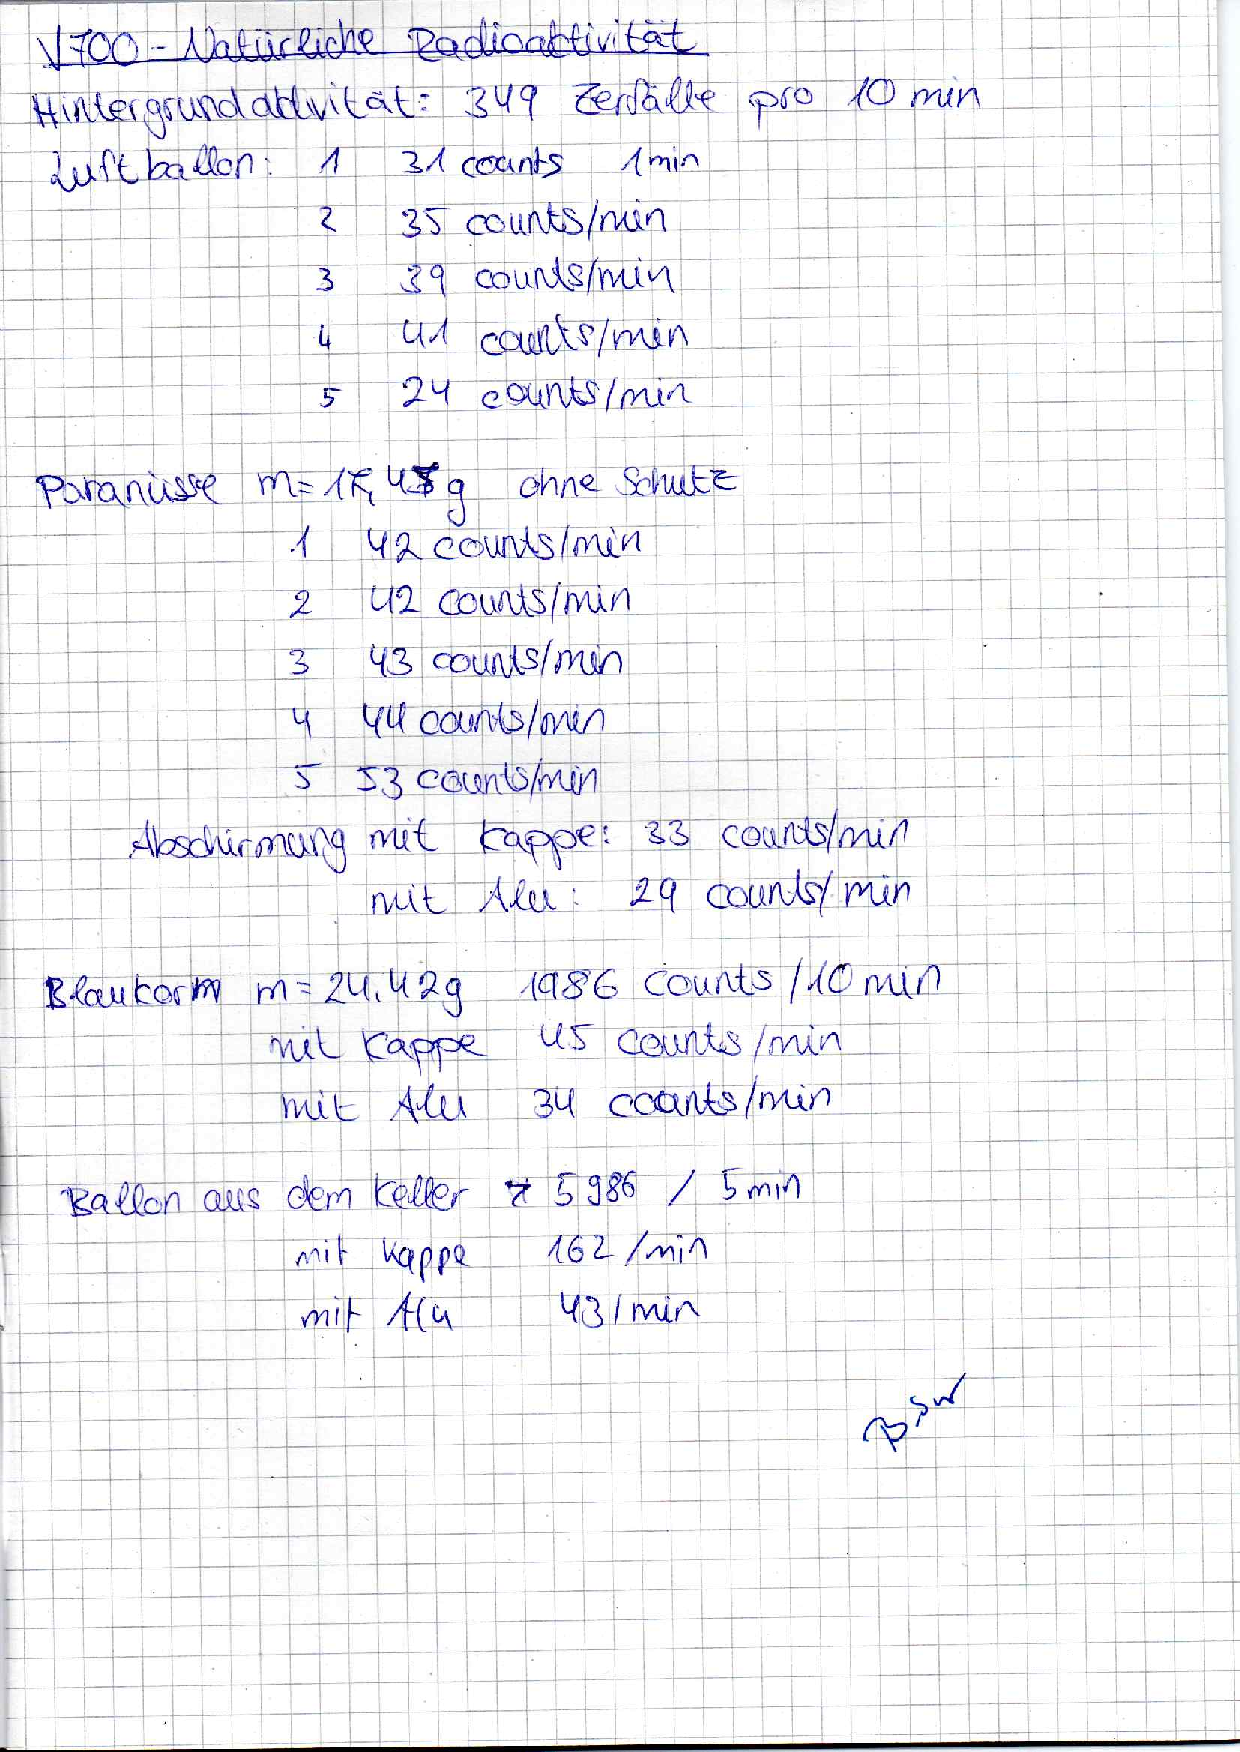
\includepdf[scale=0.7,pages=1,pagecommand=\section*{Anhang}\thispagestyle{empty}]{messdaten.pdf}
\addcontentsline{toc}{section}{\protect\numberline{}Anhang}
%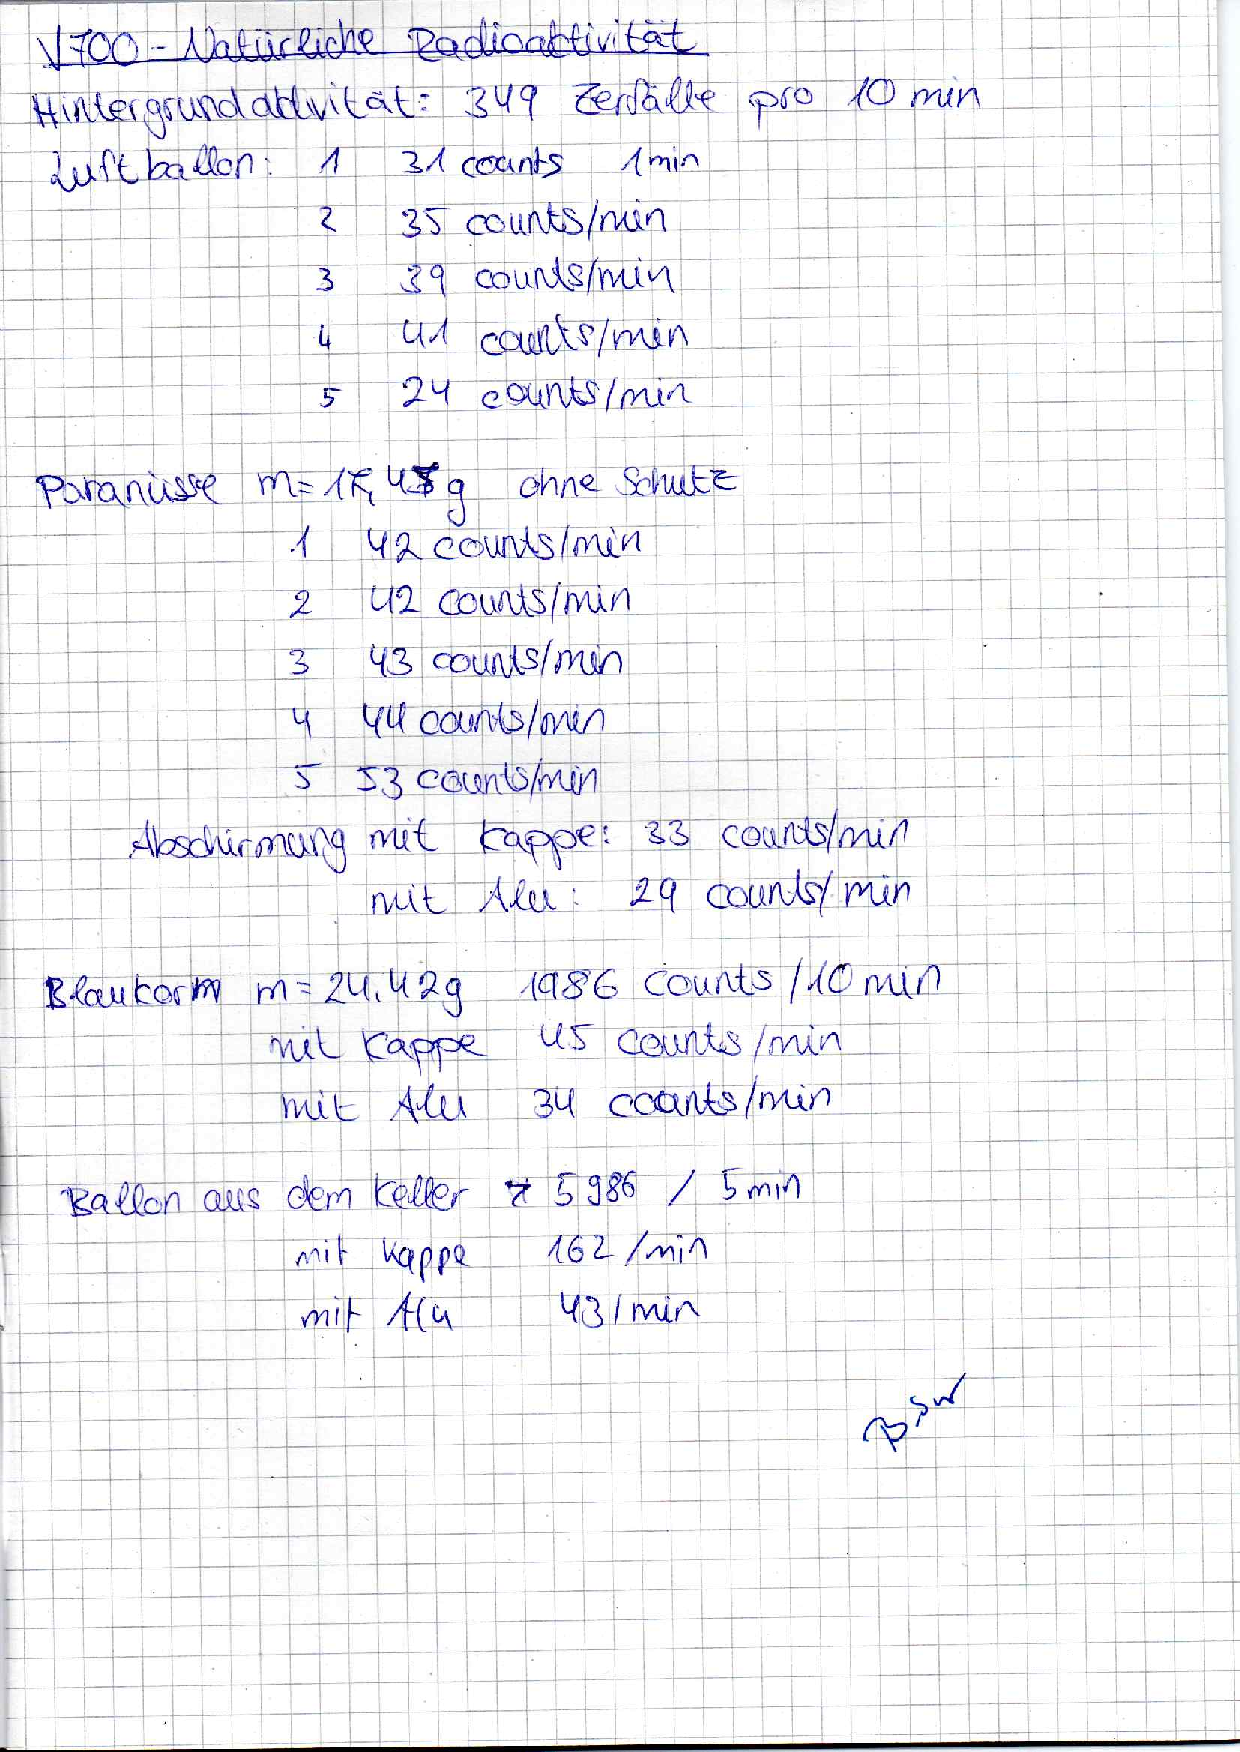
\includepdf[scale = 0.7, pages=-]{messdaten.pdf}

\end{document}
